\section{Implementation}

\subsection{Changes to the simulator}
For the implementation of the QTAR algorithm, we had to make some changes to the simulator.

\subsubsection{Hello Packet}
As far as concerns the \textbf{Hello Packet}, we made the following changes:
\begin{itemize}
    \item \textbf{Link holding timer}: the time after which a link is considered broken.
    \item \textbf{Sequence number}: the sequence number of the packet. This is used to check if a packet is a duplicate or not. We discarded this part from the paper because it will never happen in this simulator
    \item \textbf{One-hop neighbors}: each drone will attach to the hello packet its list of one-hop neighbors. This is used to update the list of two-hop neighbors of the other drones.
    \item \textbf{Two-hop neighbors}: each drone will attach to the hello packet its list of two-hop neighbors.
\end{itemize}


\subsubsection{Drone}
As far as concerns the \textbf{Drone}, we made the following changes:
\begin{itemize}
    \item \textbf{Speed}: the speed of the drone. This is used to move the drone in the environment. We modified it making it random at initialization.
    \item \textbf{Hello interval}: the time between two hello packets.
    \item \textbf{Link holding timer}: the time after which a link is considered broken.
    \item \textbf{Distance between the drones}: a list of the distances with the other drones and the time at which the distance was measured.
    \item \textbf{One-hop neighbors}: the list of one-hop neighbors of the drone.
    \item \textbf{Two-hop neighbors}: the list of two-hop neighbors of the drone.
    \item \textbf{Old one-hop neighbors}: the list of one-hop neighbors of the drone at the previous time step.
    \item \textbf{Residual energy}: the residual energy of the drone. The drones will lose energy during the simulation.
\end{itemize}


\subsubsection{Utilities}
In the utilities, we added some functions that measure:
\begin{itemize}
    \item \textbf{Delay between two drones}: the time between the moment a packet is sent and the moment it is received. This is 1 second when the drones is at the max distance (distance = communication range) and 0 when the drones is at the min distance (distance = 0).
    \item \textbf{One hop speed}: this is the ratio between the distance from the i-th neighbor drone and the delay.
    \item \textbf{Two hop delay}: this is the ratio between the distance from the i-th neighbor drone and the sum delay of the two path segments (one hop delay and two hop delay).
    \item \textbf{Required speed}: the speed required to reach the destination in the time required to reach the destination.
\end{itemize}


\subsubsection{Routing}
We made two classes, AdvancedRouting and QTARRouting, in which the latter inherits the former in order to implement the Algorithm 1 and the Algorithm 2 of the paper.
In the AdvancedRouting class, we implemented the exchange of Hello Packets between the drones and the construction of the topology.
In the QTARRouting class, we implemented the reward function, the states and actions of the drones (the relay selection algorithm)
Furthermore, in the QTARRouting class, we take as action the best drone to relay to.

\begin{itemize}
    \item \textbf{Exchange hello packets}: the drones will exchange hello packets with their neighbors.
    \item \textbf{Process hello packets}: the drones will process the hello packets received from their neighbors.
    \item \textbf{Reward function}: the reward function is the same as the one proposed in the paper. The function is defined as 
    \begin{equation}
        R = A \cdot {\textit{delay}} + B \cdot \frac{\textit{two-hop node speed}}{\textit{total two-hop nodes speed}} + C \cdot \frac{\textit{perc residual energy}}{\textit{total perc residual energy}}
    \end{equation}
    where:
    \begin{description}
        \item[delay] is the transmission delay between the forwarder and the two-hop neighbor.
        \item[two-hop node speed] is the speed of the two-hop neighbor.
        \item[total two-hop nodes speed] is the sum of the speed of all the two-hop neighbors.
        \item[perc residual energy] is the percentage of the residual energy of the two-hop neighbor ($\frac{\textit{residual energy}}{\textit{init energy}}$).
        \item[Total perc residual energy] is the sum of the percentage of the residual energy of all the two-hop neighbors.
    \end{description}

    \item \textbf{States and actions}: the states and actions are the same as the ones proposed in the paper.
\end{itemize}



\subsection{Results}
In this section, we will show the results of the implementation of the QTAR algorithm compared to the other algorithms (Georouting, Random, and our best Q-Learning algorithm, CDC-GEO, from the previous homework).
For each algorithm, we will show the average delivery ratio, the average delivery time, and the average number of relays.
For each metric, we will show the average results for the different number of drones (5, 10, \ldots, 30) using different seeds (so having different positions and paths for each of them). 

\begin{figure}[h]
    \centering
    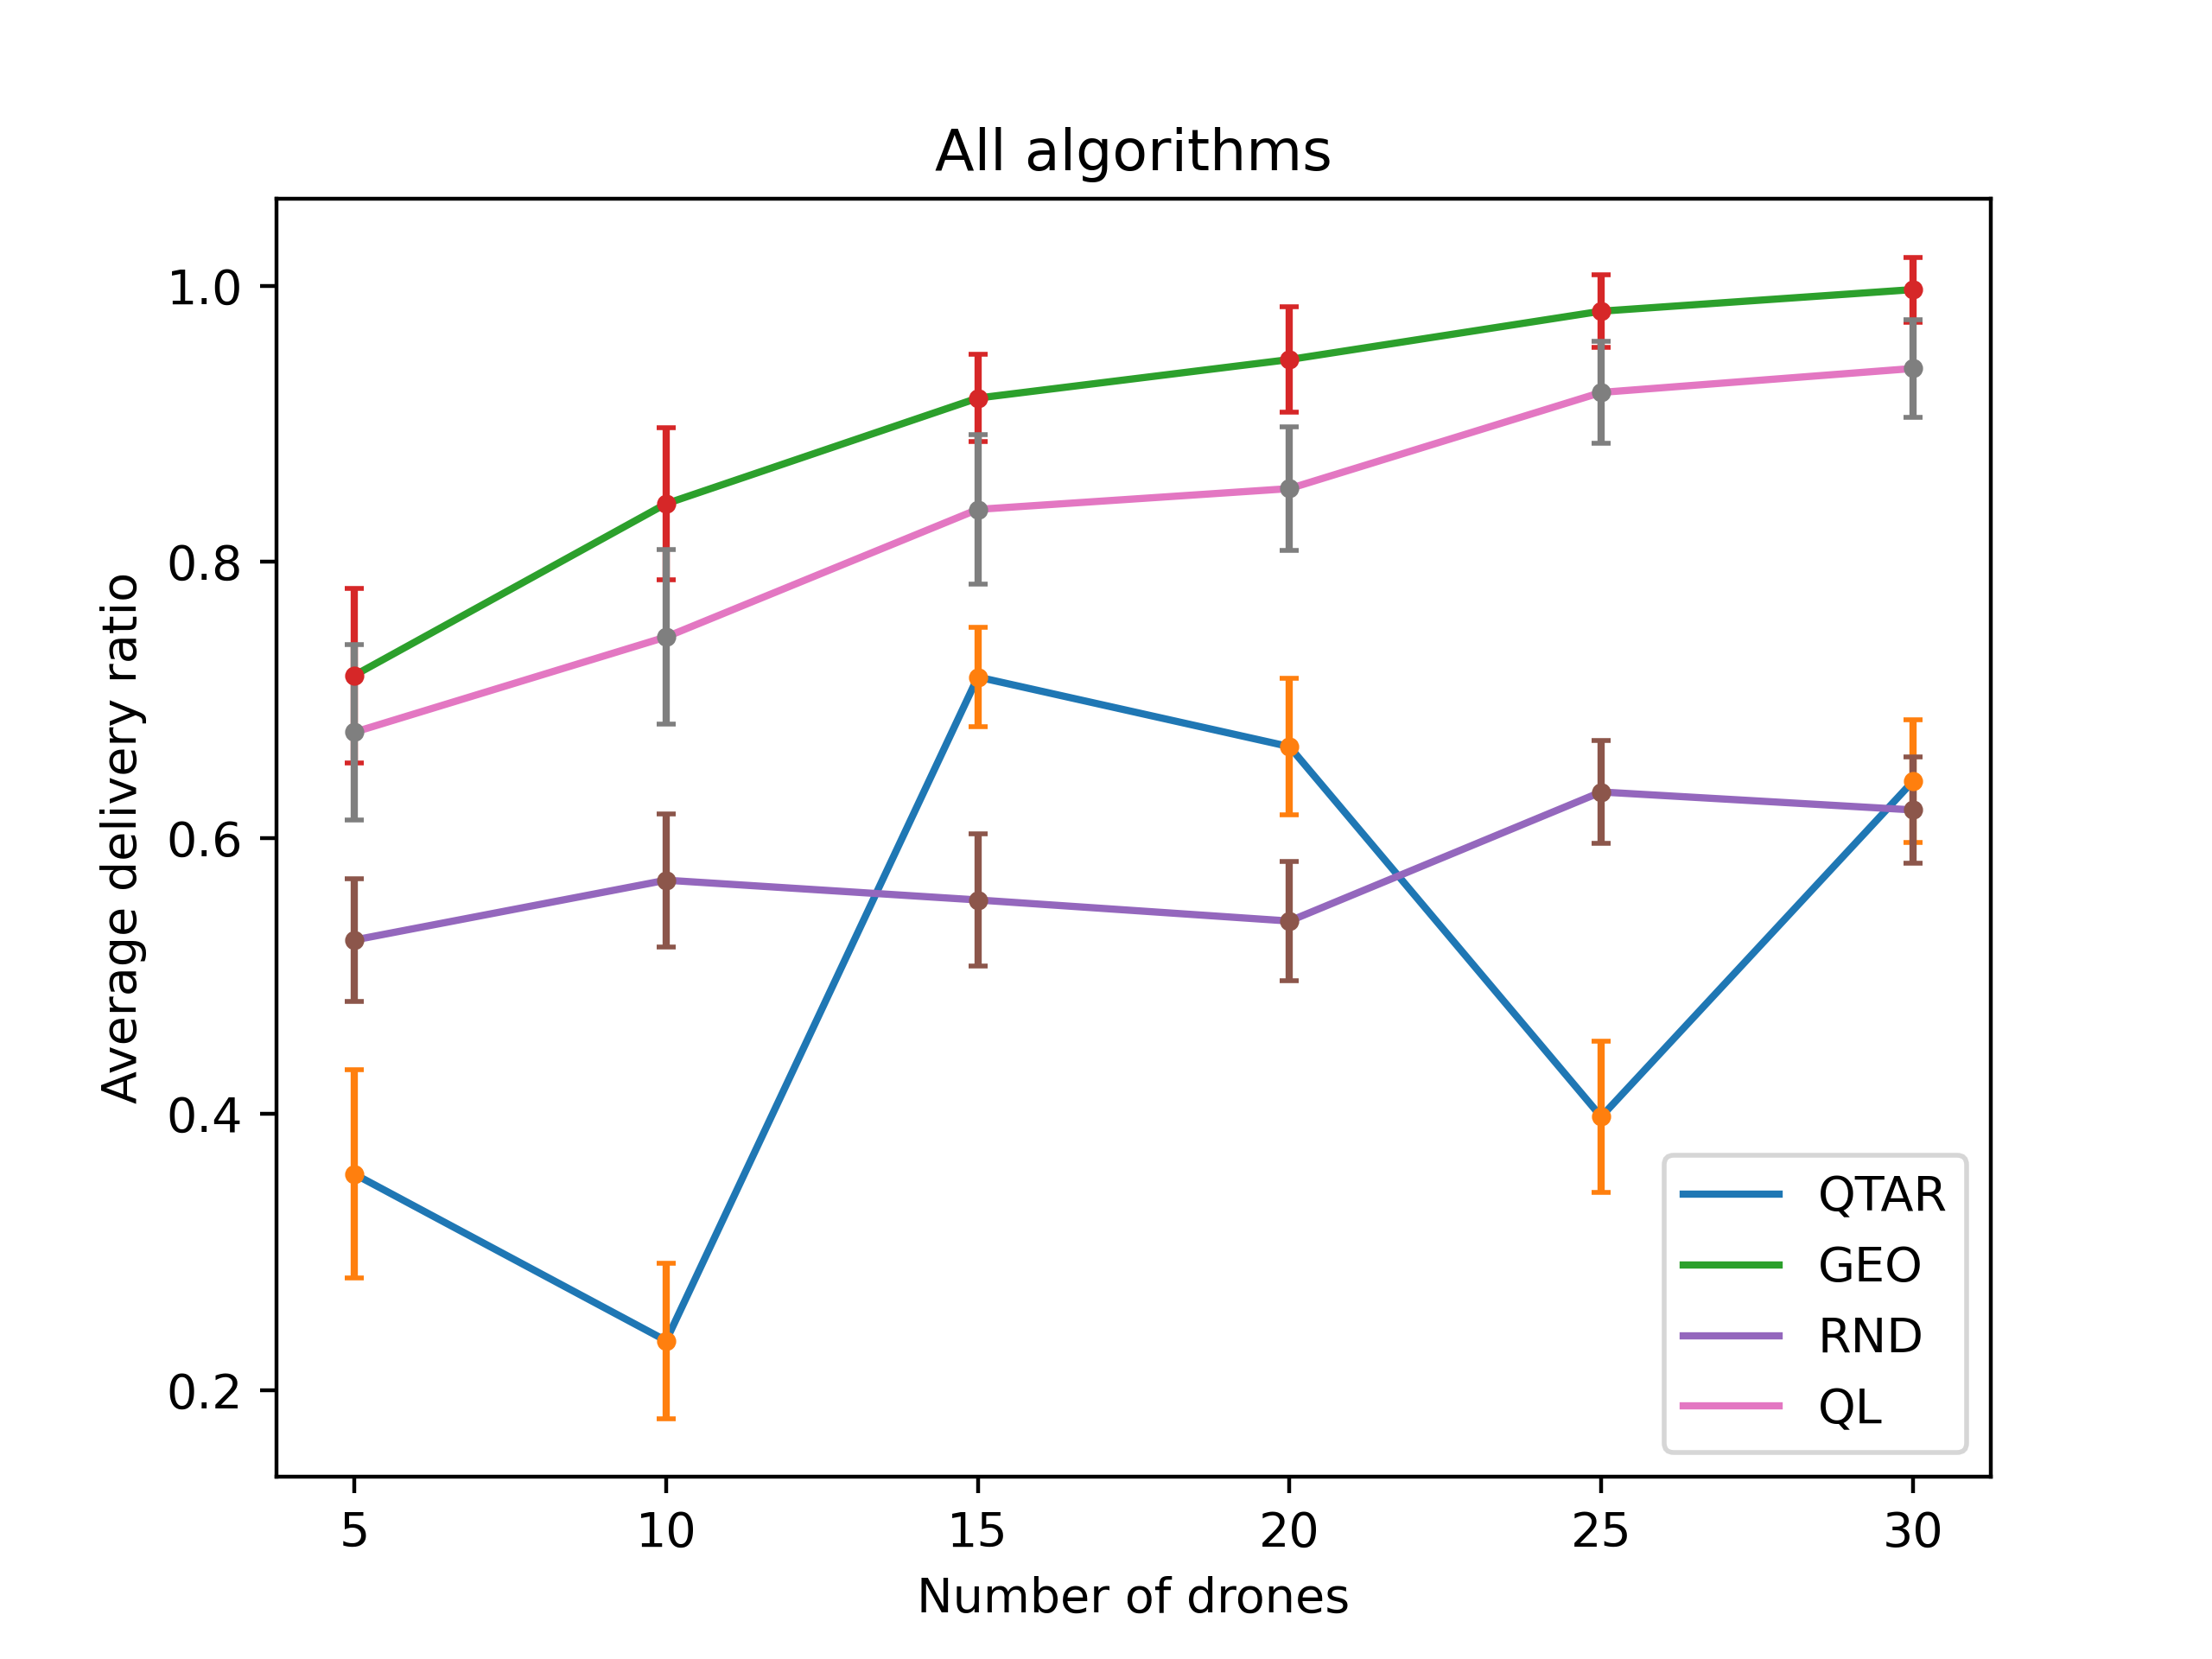
\includegraphics[width=0.7\textwidth]{../plots/average_delivery_ratio.png}
    \caption{Average delivery ratio for QTAR compared to the other algorithms}
\end{figure}

\begin{figure}[h]
    \centering
    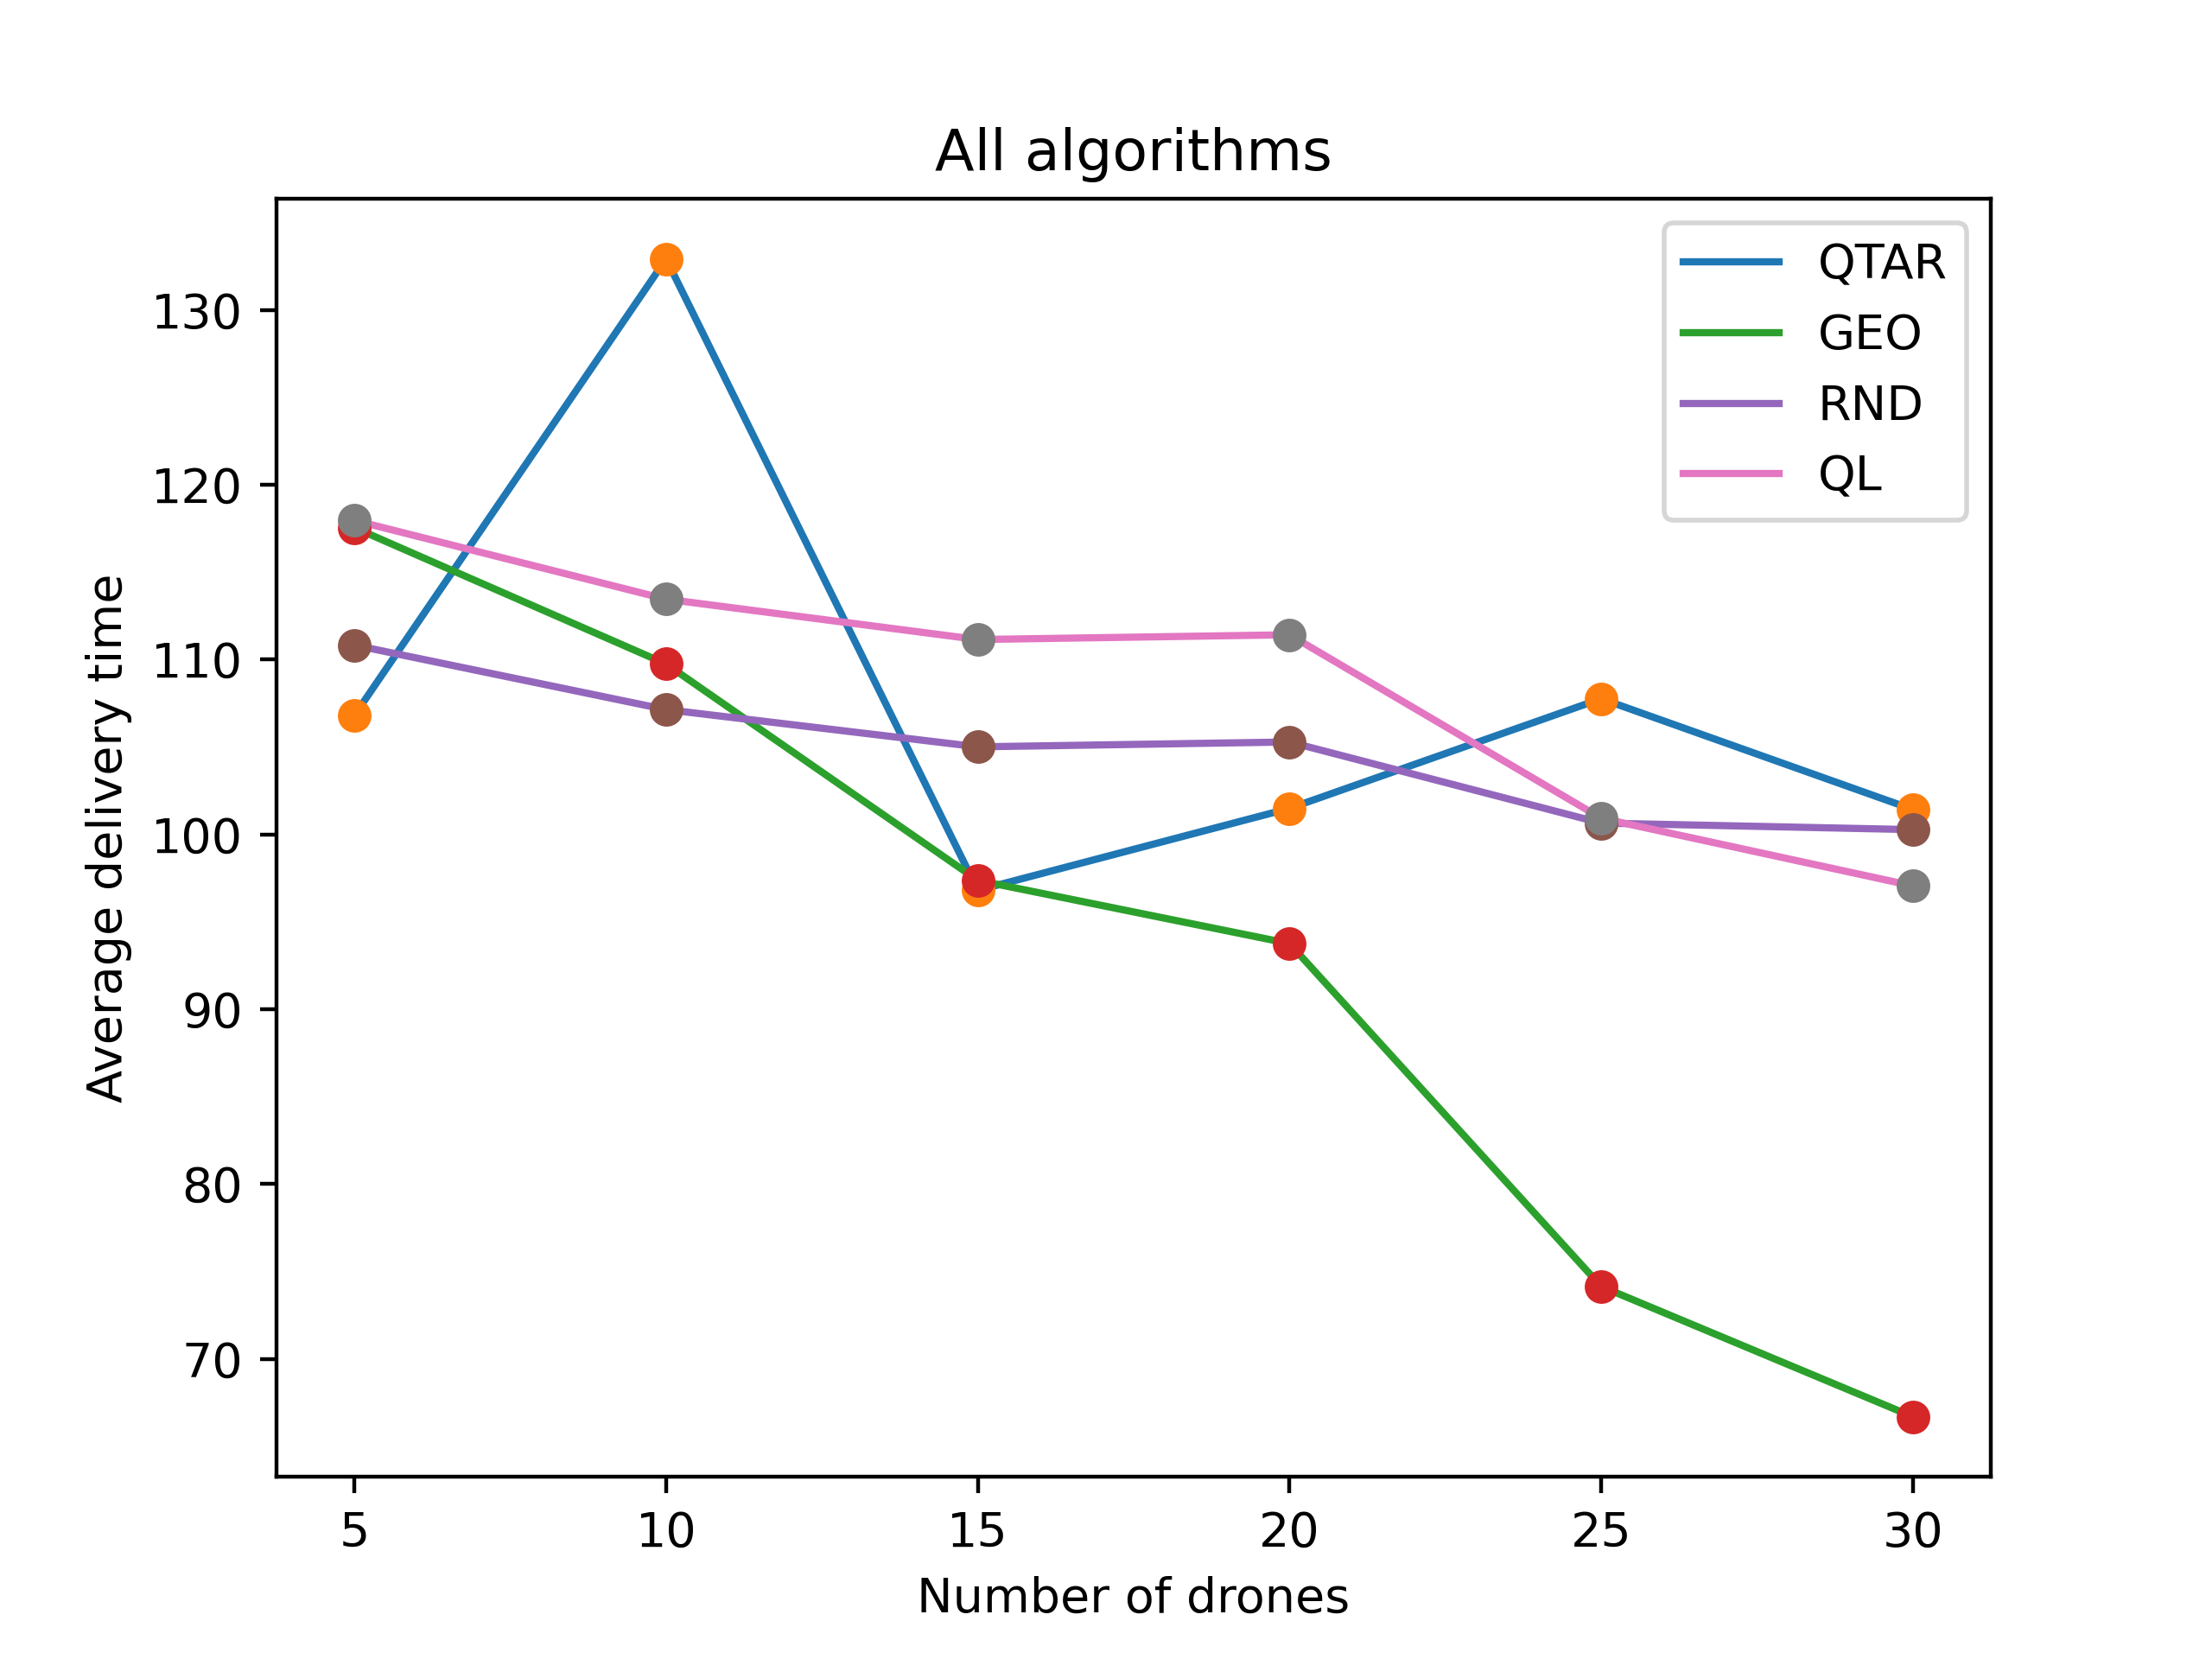
\includegraphics[width=0.7\textwidth]{../plots/average_delivery_time.png}
    \caption{Average delivery time for QTAR compared to the other algorithms}
\end{figure}

\begin{figure}[h]
    \centering
    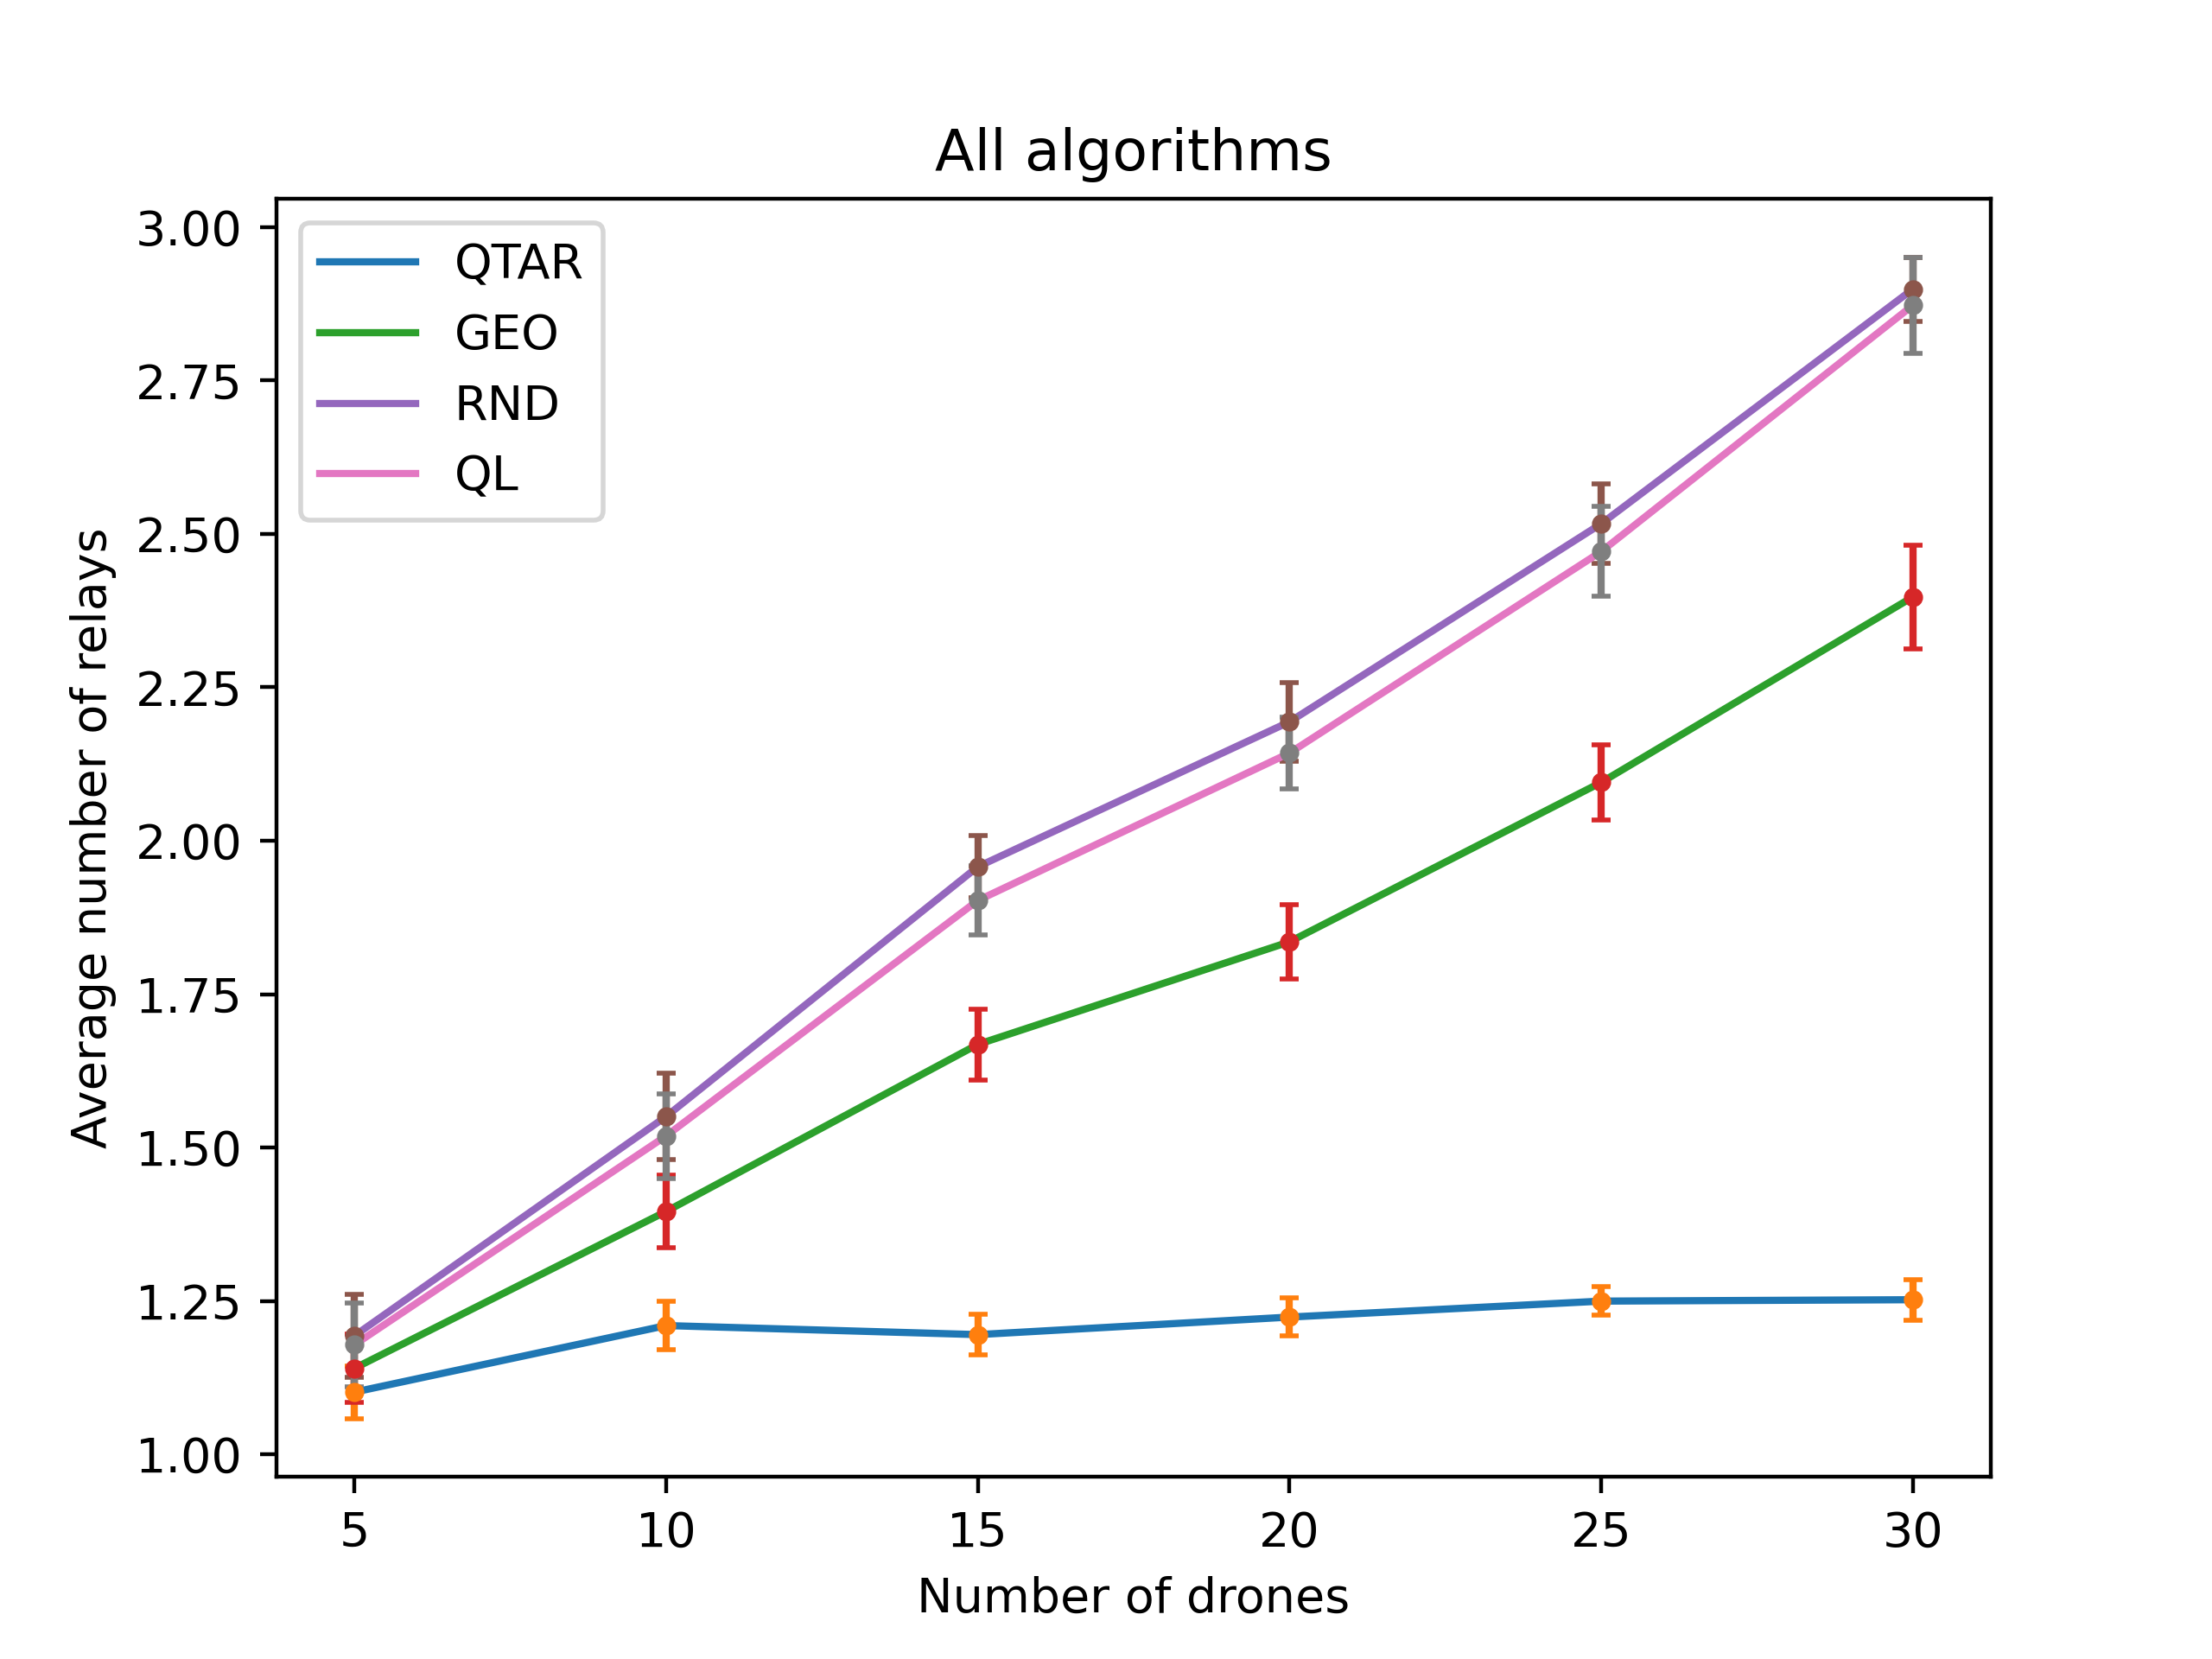
\includegraphics[width=0.7\textwidth]{../plots/average_number_of_relays.png}
    \caption{Average number of relays for QTAR compared to the other algorithms}
\end{figure}
